%many ways in which the models of previous section would manifest: effects in
%- astrophysics (only way, if dark matter only interacts gravitationally)
%- particle physics (underground, fixed target, and colliders)

The effects of the interactions described in the previous chapter have many consequences, both in astrophysics experiments, where the consequences of gravitational interactions are unavoidable, and in particle physics experiments such as underground DD experiments, fixed target experiments and detectors at particle colliders, where non-gravitational interactions must play a role. 
%why colliders (what is a collider)
%- high energy
%- very well-understood detectors 
%- not able to prove non-interacting particles are invisible particles but
%- discover/study other mediators and other particles in dark sector, not just invisible particles
%why lhc (what is the LHC)
%- interactions may be feeble because because mediator is heavy, or because couplings to SM are small
%- highest energy, able to probe highest energy scales of any collider
%- largest luminosity for hadron-hadron collisions, can reach small couplings
%- complementarity: effective coupling to hadrons required for production in pp collisions, also required for nuclear scattering in DD

To study new types of interactions, collisions of known particles at high energy, observed with very well understood detectors, have been a very successful tool, leading to the discovery of many of the fundamental components of known matter in the SM. %link is completely missing here
Collider experiments alone cannot establish that a newly-discovered invisible particle is invisible particles. But the discovery of such particles at the LHC would open up direct study of their production mechanism, such as observing the SM-invisible particles interaction mediators in other channels, and possible study of additional particle content of the dark sector. %this essentially means we are free from astroparticle uncertainties, more explicit?

The LHC, which presently collides protons at a center-of-mass energy of 13~TeV, is the highest-energy collider in operation.
Since SM--invisible particles interactions may be feeble because of a high mediator mass or small couplings, high energy and large numbers of collisions are needed to probe for them, and the LHC will deliver both in the coming years. 
In the following, we will discuss searches for invisible particles from three LHC experiments, ATLAS, CMS, and LHCb~\cite{ATLAS2008,CMS2008,LHC2008} and briefly touch on some results from previous colliders. %does ALICE search for invisible particles?
Results discussed in this review include up to 36~\ifb of proton-proton data collected up to the end of 2017, a dataset corresponding to more than three times what used for the Higgs discovery and to 1\% of the dataset expected to be collected during the full LHC run including HL-LHC. 

For each type of signature, we will discuss how the relevant searches are done, what some of the challenges are, and how the searches constrain new particle masses and interactions. 
How these constraints affect the potential signals in non-collider searches and the invisible particles abundance are separate issues, that we discuss separately in a later section, where, for example, the LHC bounds on particle properties (couplings, mediator mass, other parameters of the Lagrangian in a particular model) obtained from relativistic collisions are extrapolated to the non-relativistic collisions of invisible particles+nucleons. 

%killed: die fuckers: ATLAS, CMS, and LHCb are well placed to obtain access to high scale and rare process, planning to collect 3/ab by 2035 at the LHC design center-of-mass energy of 14 TeV. 

\begin{marginnote}[]
\entry{Run-1}{First period of LHC running (2010-2012) at 7 and 8 TeV center-of-mass energy, where approximately 20~\ifb of data were collected by ATLAS and CMS.} %this is probably too much information
\entry{Run-2} {Second, ongoing period of LHC running (2015-2018) at 13 TeV center-of-mass energy, planning to collect approximately 100~\ifb of data.}
\entry{HL-LHC} {High-Luminosity LHC running period, planned to start in 2026 to collect 3000~\ifb.}
\end{marginnote}

%transition????
%We start describing searches for invisible particles interacting through SM bosons~\ref{sec:results_ZHSearches}, then move to generic searches for signals of invisible particles with missing transverse momentum and signals of mediators decaying into visible particles~\ref{sec:results_monoXSearches}, outline the searches for complete models with invisible particles candidates in Section~\ref{sec:results_SUSYSearches} and finally conclude with searches for long-lived particles~\ref{sec:results_LLPSearches}. Throughout this chapter
%and in Section~\ref{sec:experimentalChallenges} %CD: removed in favour of sidebars
%we will highlight the experimental challenges and the novel experimental techniques used to overcome them,
%motivated by the strong interest in dark matter searches. 
%We then conclude with searches for long-lived particles within models of invisible particles in
%Section~\ref{sec:results_LLPSearches}. %CD: need to rewrite this sentence, but the idea is: if we hadn't had invisible particles as a motivation motivation we wouldn't have done this difficult stuff. 

\subsection{Searches for invisible particles production mediated by SM-bosons}
\label{sec:results_ZHSearches}

%%%%Z TO INVISIBLE

%- we are sensitive to even lighter neutrinos than 1 MeV wimps
%- we have seen Z decays decay invisibly to light and weakly interacting particles: neutrinos
%-- how have we done that? a visible + MET search (with constraint, at LEP)
%- difference between invisible particles reactions in SM and new physics models: rates 
%- constrain with total Z to invisible
%- results (numbers)

%searching for invisible particles:
%The Z boson has a fuckload of invisible decays

%main background to many other searches for invisible 

%useless info about Z 
%CD only mentioning below because it's like a monophoton
%Simple (but somehow messy) explanation in https://cds.cern.ch/record/1750933/files/CERN-THESIS-2013-330.pdf, Hugo's student
%Hugo did it, unpublished: https://www-cdf.fnal.gov/physics/ewk/2007/ZnunuWidth/
%CDF direct: 466 pm 42
%\textbf{Decays of the Z boson into invisible particles} can be constrained using the invisible Z width. It can be measured directly in Z decays in association with a photon emitted as initial state radiation. Events are selected containing a single photon, missing transverse momentum and no other sizable event activity. This selection is also used for identifying events from possible invisible particles reactions at colliders.
%LEP combined: 503 $\pm$ 16 MeV
%The total Z width has been measured indirectly at LEP~\cite{ALEPH:2005ab} leading to a measurement of the number of light neutrino families compatible with cosmology; if the partial widths of the decays into visible particles are subtracted from the total width, the invisible width can be measured to 499.1 $\pm$ 1.5 MeV~\cite{Patrignani:2016xqp}. 
%The precision of the indirect measurement is better than that of the direct measurement, due to the higher statistics and the relative ease of selection and background subtraction for the visible Z decays. %CD: omitted, no space
%The main systematic uncertainty in this case comes from the theoretical uncertainties in the simulation. CD: Carena seems to think it is an uncertainty on fast simulation
%\begin{marginnote}[]
%Direct and indirect Z width measurements must agree if the decay of the Z to a pair of invisible new particles is to be the main mechanism responsible for the deviation from the SM values. 
%\end{marginnote}%CD: I think this is important to mention in the same sense as the caveats on the s-channel resonances, but it can be omitted
%in this case, an analysis of the mass of the system recoiling against the photon would provide a handle to distinguish between different BSM processes. %CD: omitted because this is possibly too handwavy but how can we summarize 4 pages of Carena in a sentence?
%Carena quantitative: At present, measurements at LEP and CHARM II are capable of constraining the left-handed Z\nu\nu-coupling, 0.45 <~ g_L <~ 0.5,  while the right-handed one is only mildly bounded, |g_R| <= 0.2.

There is already spectacular evidence from high-energy colliders for copious production of low-mass invisible particles mediated by the Z boson: the huge rate of neutrino production. 
The invisible production rate via the Z boson is often the largest background to searches for invisible particles produced through other means, and is therefore important to understand very well.
The rate itself would differ from the predictions of the SM if the Z boson couples to additional invisible particles lighter than about half its mass.
The most precise measurement of the invisible Z width, 499.1 $\pm$ 1.5 MeV~\cite{Patrignani:2016xqp}, has been inferred from the total width at LEP~\cite{ALEPH:2005ab}. This can be used to constrain the parameters of new physics models where the Z decays to new invisible particles, such as Z portals~\cite{Carena:2003aj,Arcadi:2014lta,Escudero:2016gzx}. The coupling between the Z and an invisible Dirac fermion is constrained to be smaller than 2-3\% for invisible particles that are significantly lighter than half the Z mass.
A less-precise direct measurement, also by LEP, uses invisible Z decays in association with a photon emitted as initial state radiation (ISR).
Selected events contains a single photon, missing transverse momentum and little other event activity. This \MET+ISR is a key signature for invisible particle searches at colliders. 
At the LHC, precision measurements of the production and decay of Z bosons can be used to continue testing for the effects of invisible particles in the electroweak sector. 
For example, a measurement from ATLAS of the ratio of cross sections of events containing a jet and \MET, dominated by invisibly-decaying Z bosons, and events where the Z boson decays into an opposite-sign, same flavor dilepton pair, is sensitive to the anomalous production of invisible particles~\cite{Aaboud:2017buf}. 

The Z boson is also key to the invisible decays of the newly-discovered Higgs boson. These Higgs decays contribute to less than 0.1\% of its total decay width in the SM, dominated by the small rate of Higgs decays to a pair of Z bosons that then both decay invisibly. The LHC cannot directly measure the Higgs total width in a model-independent fashion\cite{Dobrescu:2012td}, and its small width to invisible particles in the SM is far below current experimental sensitivity, so an observation of invisibly-decaying Higgs would imply new physics. 
Searches at the LHC either attempt to directly observe the invisible decays of the Higgs boson, via its recoil against visible particles, or compare measurements of the Higgs parameters with their precise theoretical calculations. 
Higgs to invisible LHC searches using Run-1 and Run-2 data employ and combine different Higgs production modes and decays. In all cases, in addition to a requirement of sizable missing transverse momentum, auxiliary visible objects are used to select the events. Decays into invisible particles would reduce the SM Higgs production and decay coupling strengths~\cite{Khachatryan:2016vau,Englert:2011yb,Aad:2015pla}, making precision measurements important to test the presence of new Higgs decays. Combining direct and indirect searches, the most stringent upper limit on the fraction of invisible decays of the Higgs boson is 23\%~\cite{Khachatryan:2016whc,Aad:2015pla}, setting constraints on Higgs portal model couplings of 1-2\% for Dirac invisible particles much lighter than half the H mass. 
%For the Higgs boson, the upper limit on the branching fraction to visible and/or invisible non-SM particles only using precision measurements is 34\%

\subsection{Generic searches for invisible particles from BSM mediation}
\label{sec:results_monoXSearches}

Searches for invisible decays of Higgs and Z through Higgs and Z portal models can be seen as tailored instances of more generic searches for BSM mediation of invisible particles. 
The mediator mass plays a role in the LHC phenomenology. The invisible particles are decay products of Z and Higgs, therefore the amount of \MET in the event is limited due to the electroweak 
scale mass of these mediators, and known properties of Higgs and Z bosons are exploited to reject backgrounds. The constraints from these searches are limited to masses of the invisible particles below 40-60 GeV. In order to reach larger mediator and DM masses, a more generic and broader set of searches are employed across a variety of different signatures. 

\begin{textbox}[!h]
\section{Measuring invisible particles: \MET reconstruction}

%10 words per line, 20 lines
%While at lepton colliders the initial center of mass energy is known and 
%can be used as an additional constrain to measure the momentum imbalance due to escaped invisible particles in the final state, measuring missing transverse momentum at hadron colliders
% TJ: Not sure why you make this distinction?
% I tend to think about the lepton collider case as offering
% one extra constraint, i.e. on the total missing *energy*
% but the directional MPT constraint still requires an
% inclusive measurement
Precise measurements throughout each detector systems are crucial to measure \MET in experiments at hadron colliders. This is because the calculation of \vec{\MET} should include all particles in the event.
% regardless of whether they are reconstructed as physics objects (jets, electrons...). 
Contributions that are not attributed to physics objects form the soft component of the \MET~\cite{Aad:2016nrq,CMS-PAS-JME-16-004}. 
One of the main challenges for \MET measurements are excluding contributions other than the hard-scatter process, e.g. from pile-up. 
Searches for invisible particles also need to efficiently reject events with large \MET if the visible energy is due to non-collision background. 

\textbf{Challenge: pile-up in \MET reconstruction.} 
%Momentum contributions from additional proton-proton interactions can have a significant contribution to the overall transverse momentum balance.
In addition to the pile-up suppression techniques applied at the calorimeter level, tracking information can be used to determine whether energy deposits originate from the primary collision vertex. 
The combination of this information is used to remove pile-up both in the physics objects used for \MET calculation and in the overall event energy balance~\cite{CMS-PAS-JME-16-004,ATLAS-CONF-2014-019}. 
%Trigger rates grow exponentially with the number of additional interactions

%[cite: https://cds.cern.ch/record/2205284/files/JME-16-004-pas.pdf, asked Emma and TJ for best reference]
%The lack of tracking information in the trigger system is a limiting factor in selecting events with low \MET at the trigger level, as the rates grow exponentially with the number of additional interactions. 
%from https://twiki.cern.ch/twiki/pub/AtlasPublic/MissingEtTriggerPublicResults/metxs_vs_mu.pdf

\textbf{Challenge: fake \MET rejection.} 
Non-collision backgrounds, such as cosmic rays, beam background and detector noise have a significant contribution to the tails of the \MET spectrum, as shown in Fig.~\ref{fig:fakeMET}
Specific quality cuts, based on the presence of tracks associated to the deposited energy and on energy deposited in the various calorimeter layers are applied to reject these events~\cite{ATLAS-CONF-2015-029}.~\footnote{The number of events passing the jet+\MET analysis selection before these quality cuts is about ten times larger than the SM contribution~\cite{Aaboud:2016tnv}.}. 
\end{textbox}

%Maybe move this to chapter 3

%\subsubsection{Missing transverse momentum}
%\label{sub:MET} 

%Main points:
%\begin{itemize}
%\item The measurement of \MET relies on the precise measurement of all reconstructed physics objects. 
%\item Some description of \MET significance may be needed, but it may also be too academic. 
%\item Fake \MET is rejected using quality cuts.  
%\item Pile-up needs specific techniques because of the soft terms. 
%\item \MET at the trigger level is the driving reason why we can't go lower, see next section.
%\end{itemize}

%from ooutline

%- Mismeasured MET (combining instrumental effects and beam/cosmics background)				
%	- CDF				
%		- beam background: exploit track pointing to jet and calorimeter layers				
%		- QCD: shitty method from Mario (extrapolation changing the veto)				
%	- LHC:				
%		- beam backgrounds: like CDF, more refined				
%			- can have a % of how many events would have been				
%		- QCD: matrix method a la SUSY				
%	- Other backgrounds (diboson, top)				
%		- Small so using MC				
%		- LHC has validation regions				
%			- check ttbar				

%Valerio's talk for relevant plots 
%https://indico.cern.ch/event/466934/contributions/2590281/attachments/1489278/2314178/20170706_EPS_invisible particlesatATLAS.pdf

%MET significance: in VBF CMS search
%For the 8 TeV dataset, an additional requirement is set on an approximate missing transverse energy significance variable S(Emiss) defined as the ratio of Emiss to the square root of the scalar sum of the transverse energy of all PF objects in the event [62]. Selected events are required to satisfy S(Emiss) > 4?GeV.

Many collider searches for invisible particles aim to be model-agnostic. They seek anomalous events consistent with invisible particles being produced, identified by presence of one or a few visible objects recoiling against them, and are designed to detect an excess of \MET over the SM background. 
This has remained the aim of invisible particle searches as center-of-mass energy and dataset size have increased, from LEP to Tevatron to the most recent LHC searches~\cite{Fox:2011fx,Beltran:2010ww,Bai:2010hh}.
Here we discuss these searches, often called 'mono-X' searches, although the radiation of a single object is only the leading process in the reaction~\cite{Haisch:2013ata}. 
We start with the 'jet+\MET' search, which exemplifies many of the challenges and techniques used in other general invisible particle searches.

%We begin this section by describing the LHC searches for missing transverse momentum in association with one or more hadronic jets. The jet+\MET search allows us to illustrate many of the techniques used in invisible particle searches, and it is one of the most powerful to constrain BSM-mediated simplified models of invisible particles. We then move on to outlining searches using different associated objects, and continue with searches for visible mediators that are the consequences of the invisible particles production mechanism. Finally, we compare and discuss the sensitivity of invisible invisible particles and visible mediator searches at the LHC. 

\subsubsection{Searches with jets}

%- searches for invisible particles (where the interaction is mediated by another particle) all have a common denominator in the large Z + (stuff) to invisible SM background
%- for H and Z we know signature is relatively low MET
%- with BSM mediators, we don't: looking in different slices of phase space (different MET regions) with different associated particles (different signal/background ratios and sensitivity to particular operators)

%Can think of searches for H->invisible and Z->invisible as tailored instances of more generic searches where mediator can be whatever the fuck. Invisible signals for masses above 45-60-ish GeV; up to half mediator mass. So: much wider range of the amount of MET is possible. So while the H-invisble searches are tailored to a particular range of mediator masses (90-125 GeV), a more generic set of searches, often termed 'mono-X' searches, are performed to probe this wider variety of signatures found in the BSM mediator models.

One way to approach [this, the goal of model-agnosticism] is to require that the recoiling visible particles are produced by SM processes, not in the dark interaction. ISR meets this criteria. SM bosons are likely to be present in any BSM process, radiated from initial state partons at rates fixed by the SM. Because gluon ISR is far more prevalent than the other forms, the jet+\MET search is important particularly when the details of the dark interaction are unspecified.

Since the presence of highly energetic invisible particles would manifest as an excess of events with a significant \MET, the main observable for this search is the number of events in \MET \textit{signal regions}, either exclusive (in bins of \MET) or inclusive (considering all events above a given \MET threshold). 

To look for signal, the jet+\MET search selects events with a moderate amount of \MET (in the 13 TeV analyses, typically above 200 GeV) and at least one jet with \pt larger than 100-200 GeV in the central region of the detector ($\eta<2.4$). 
%with \pt $>$ 250 GeV (ATLAS) or \pt $>$ 100 GeV (CMS) and \MET $>$ 250 GeV (ATLAS) or \MET $>$ 200 GeV (CMS). 
These \MET and jet \pt thresholds are set in order to achieve a manageable data-taking rate for these events. Selecting events (triggering) in a model-agnostic way is a challenge for models that do not produce a large amount of \MET, because one is forced to assume more about the visible recoil. 

%This selection ensures that all events with these characteristics are recorded by the trigger system for further analysis. Events with lower \MET suffer from higher instrumental and SM backgrounds, which prevents the whole event sample from being recorded due to storage limitations. 

\begin{marginnote}[]
\entry{Trigger}{a detector system that decides which LHC collision events are to be recorded for physics analysis. For a description of the trigger systems of the ATLAS and CMS experiments, see ~\cite{Smith:2016vcs,Aaboud:2016leb,Khachatryan:2016bia}.}
\end{marginnote}

%Searches for invisible particles presents different challenges, depending on the invisible particle mass and boost. If the mediator is heavy, any light invisible particle will receive a boost and appear as an excess in the tails of the SM \MET distribution. If instead the invisible  particle pair originates from a light mediator, of the same mass range as the Higgs boson, it will manifest itself at low \MET. The low \MET suffers from a much higher rate of both instrumental and SM backgrounds.
%As a consequence, it is impossible to record and store all events with a low-\MET for further analysis, since at the data-taking stage (within the \textit{trigger} and data acquisition systems) it is difficult to obtain further handles to discriminate signal and background, and the sensitivity to low-\MET signals is compromised. This challenge will be discussed further for both visible and invisible particle searches in Sec.~\ref{sub:twoBody}.

\begin{marginnote}[]
\entry{Signal region}{a region of phase space for a search that is enriched in signal events. Event counts in this region are used to compare background-only prediction to data in search for discrepancies signaling new physics. 
%For example, a region with a high \MET and no other objects except for the ISR object is a signal region for a \MET+X search.
}
\entry{Control region}{a region of phase space for a search that is signal-free but with characteristics otherwise as close as possible to the signal region. Event counts in this region are used to estimate backgrounds in the signal region. 
%For example, a region requiring no \MET and a process mimicking that of the signal region is a control region for a \MET+X search.
}
\end{marginnote}

%List of backgrounds & cut

From this sample of events, these searches typical further restrict how many hadronic jets and additional visible particles may be present, in order to suppress contributions from SM processes and instrumental backgrounds that can exhibit significant \MET. These requirements reduce the generality of the analysis to an extent but also better isolate signal-like events.
For example, vetoing events with leptons suppresses contributions from W bosons decaying to leptons. 
SM multi-jet processes can exhibit large \MET when one or more jets is mismeasured. Such mismeasurements often result in the \MET pointing in a similar direction as the jet, and this feature is used to reduce this background to about 1\% of the total.
%$\phi$ direction of the missing transverse momentum vector does not align with the direction of the four-momentum of the jets with the highest \pt (leading jets).
%The remaining QCD background estimated from data amounts to less than 1\% of the total background. 
Non-collision events (e.g., intersecting cosmic rays, beam-gas interactions, and calorimeter problems) can also create spurious \MET.
These backgrounds can overwhelm the search, and [much work can go] into designing criteria to identify them. 
Fig.~\ref{fig:fakeMET} are rejected with specific quality criteria.%Sidebar? Textbox?
A restriction on the number of jets above a certain threshold rejects backgrounds from top production. 

The result is a sample consisting mainly of invisible decays of the Z boson (approximately 55-70\% of the total background).
%CMS excludes taus, while ATLAS does not. Too much detail imo. 
%numbers in Livia's talk: https://indico.cern.ch/event/682235/contributions/2817876/attachments/1576792/2490208/invisible particlesWG-2017_V2.pdf and in Francesca's talk:
%https://indico.cern.ch/event/682235/contributions/2817877/attachments/1576793/2490236/171218_atlas_ungaro.pdf
and leptonic decays of the W boson where the lepton is not
reconstructed (approximately 20-35\% of the total background), in association with jets.

\begin{figure}[!htpb]
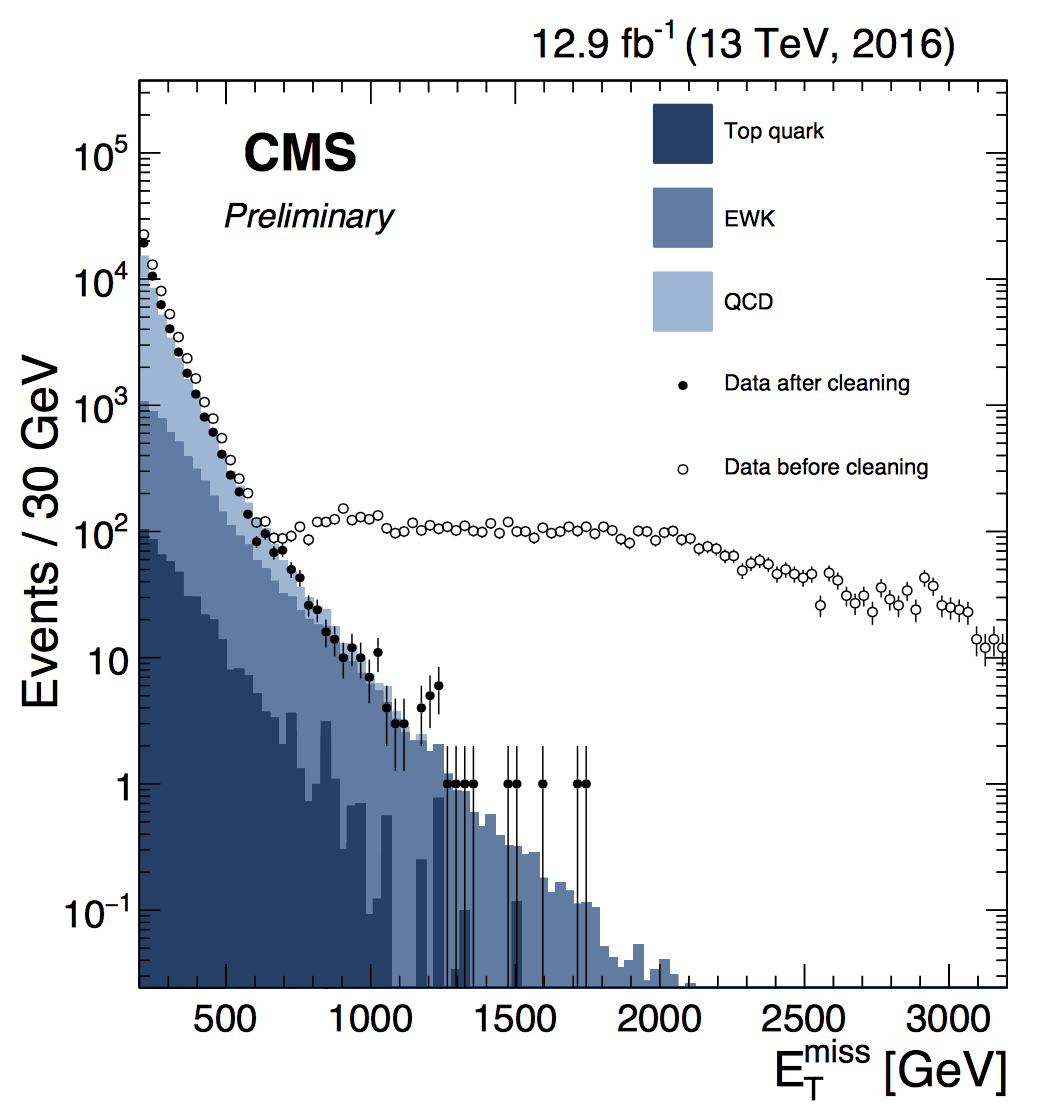
\includegraphics[width=0.5\textwidth]{figures/FakeMETTemp.png}
%Caption from the ATLAS monojet but they only have pT
%https://atlas.web.cern.ch/Atlas/GROUPS/PHYSICS/PAPERS/EXOT-2015-03/
\caption{The \MET distribution of events in data, selected using criteria of high total hadronic energy ad at least two jets with \pt{} $>$ 400 and 200 GeV (open markers), from simulation (filled markers) and
after applying fake \MET rejection criteria.  
%data events passing the [define selection] without any cleaning criteria applied on the leading jet. The Standard Model background indicated in the plots corresponds to the estimates obtained for the analysis signal region, including jet quality requirements. 
%The jet selection inefficiency of the cleaning selection is O(1\%), which is negligible compared to the observed excess in data. 
This demonstrates the necessity of a strong non-collision background suppression for jet+\MET-type analyses. From~\cite{CMS-PAS-JME-16-004}.}
\label{fig:fakeMET}
\end{figure}

%CMS: up to 4 leading jets 
%The CMS analysis also applies specific vetoes for photons and heavy flavour jets, to reject events with photon ISR or containing top quarks. The CMS analysis also includes a signal region targeting hadronic decays of the W and Z bosons using substructure techniques, which is considered separately in the case of ATLAS and will be discussed in Sec.~\ref{subsub:monoV}. 
%Estimating the background
%In order to reduce theoretical and experimental uncertainties on the main backgrounds, 
%
%big picture:
%- need a very precise estimate of the shape
%- calculations of this shape in QCD cannot be done to high enough order to get arbitrarily good precision
%- so predictions from available high order calculations are combined with data in the visible CR to blah.
%- combined means: use Zll as estimate of the shape, compare to MC, and correct for instrumental and other known effects.

High-statistics jet+\MET searches need a very precise estimate of the shape of the background events to be sensitive to signals of feebly interacting particles. 
As an example, the integrated number of signal events with a \MET below 510 GeV amounts to less than 0.03\% of the background~\cite{Sirunyan:2017jix}. 
%>>> 162+130+98+85+65+53+54+41
%688
%>>> 136863+74340+42540+25316+15653+10092+8298+4906
%318008
%>>> 688./318008
%0.002163467585721114
A background estimation solely from simulated events is not precise enough, due to uncertainties on both theory and detector simulation affecting the total cross-sections. 
For this reason, the \MET distribution combines information from both data and the most recent perturbative calculations~\cite{Lindert:2017olm}.
The shape of this distribution is taken from simulation, but its normalization is derived from data in signal-free \textit{control regions} selecting  visible boson+jet processes (W, Z, $\gamma$) 
where the transverse momentum of the visible decay products is subtracted from the total transverse momentum balance to obtain a proxy of the \MET distribution. 
%V+jet processes where the W and Z bosons decay into visible particles ($Z\rightarrow ll, W\rightarrow l\nu+jets$, where $l$ = $e, \mu$). 
%not sure we should say that the bin by bin estimates are used, here it's ambiguous
%The event selection follows that of the signal region, substituting a lepton requirement to the lepton veto in case of vector bosons. 
[Consider adding more info about QCD/QED correction and importance thereof, citing Ellis's paper on UA1 discovery~\cite{Ellis:159861}].
%The estimation of the number of $Z\rightarrow \nu\nu$events from the $\gamma$+jet and  $W\rightarrow l\nu$+jets control region needs a specific treatment due to the difference in the processes. This is particularly important for a consistent treatment of the different processes used in the background estimation and of the main theoretical uncertainties. %CD: how do we call the thing
%The full information on the theoretical and experimental uncertainties and their correlations from this procedure is used in a simultaneous fit to control and signal regions, to determine the overall background estimate in each of the \MET regions considered. 
%and leads to an improvement of 40 to 50% in the search according to PhilHarris and Livia, but I wouldn't add that unreferenced
Backgrounds from top processes in ATLAS are estimated using a dedicated control region with a requirement of a $b-$jet that is included in the fit, while CMS takes this background from simulation. Smaller diboson backgrounds are estimated from simulation. 

%%Experimental uncertainties
The systematic uncertainties on the background estimate for the jet+MET search range from 2 to 7\% (CMS) and 2 to 10\% (ATLAS), depending on the \MET range. The main uncertainties are due to the identification of leptons (CMS) and the understanding of the jet and \MET calibration (ATLAS). 

%- our observable is the rate, then we convert that rate to the parameters of the model: couplings, given masses
%- model-independent as a function of MET cut
%- simplified models and Higgs portal
%  - couplings for different models
%  - Equally sensitive to 

%Model-independent
Having observed no excess over the estimated background, 95\% CL limits are set on the production cross-section of invisible particles, typically spanning from 0.5\pb to 2\fb depending on the \MET threshold~\cite{Aaboud:2017phn}. 
The jet+\MET search can constrain a wide variety of interactions involving invisible particles. Therefore, various approaches have been taken to allow others to easily reinterpret its results. 
As for most LHC searches, the published experimental data from the ATLAS and CMS collaborations is provided on the HEPData platform~\cite{Maguire:2017ypu}. 
Additionally, a simplified likelihood function encapsulating the result~\cite{Collaboration:2242860}, is provided by CMS~\cite{Sirunyan:2017jix}.
%which under certain assumptions approximates the full likelihood using a reduced set of information, 
%and has been used for reinterpretation~\cite{Pobbe:2017wrj}. 
The upper limits on the rates provide bounds on interactions, not necessarily on the masses and other properties of the invisible particles themselves.
ATLAS and CMS jet+\MET results from LHC Run-1, as well as the Tevatron, also constrain EFT models.  
At the LHC Run-2, constraints can be interpreted as limits on the interactions between the mediator and the SM (e.g.\gq) under specific sets of model assumptions. 
For example interactions between (axial-)vector mediators and invisible particles with a coupling \gdm=1 can be constrained up to mediator masses of 1.5--1.9~TeV~\cite{Aaboud:2017phn,Sirunyan:2017jix}. SM couplings of order 0.1 can be constrained for lighter (axial-)vector mediators. 
Jet+\MET searches with the full 2015+2016 Run-2 LHC datasets are beginning to be sensitive to lower-rate interactions with invisible particles mediated by (pseudo-)scalar mediators. 
Limits are also set on colored scalar mediators. For unit couplings and invisible particle masses of up to 100 GeV, the mass of the mediator is constrained to be above 1.7 TeV~\cite{Aaboud:2017phn}. 

\subsubsection{Searches with photons and vector bosons}
\label{subsub:monoV}
%monophoton, monoV

%What we wrote above
%One way to approach the [goal of model-agnosticism] is to require that the recoiling visible particles are produced by SM processes, not in the dark interaction. ISR meets this criteria. SM bosons are likely to be present in any BSM process, radiated from initial state partons at rates fixed by the SM. Because gluon ISR is far more prevalent than the other forms, the jet+\MET search is important particularly when the details of the dark interaction are unspecified.

%- many other searches with ISR+MET
%-- not the higher signal xsec
%-- interesting because they are lower xsec but also higher S/sqrt(B) 
%-- when the details of the dark interaction matter these can be enhanced (VVchichi) 
%-- even for a fixed model, if this is the subdominant channel, different (lower) trigger thresholds. looking for other ISR bosons or additional particles allows lower thresholds and more acceptance for signals 

%i like this part because motivation
Besides the gluon, other particles can constitute the visible-particle recoil against invisible particle production. In the model-agnostic case discussed above, where the recoil arises from ISR, the rates for photon and electroweak boson radiation are much smaller than for gluon radiation. Nevertheless, searches in these other channels can play a complementary role, since they select a smaller and different mix of backgrounds, and are affected by different systematic uncertainties, than the jet+\MET search. Moreover, because of the lower backgrounds, events can be recorded with lower kinematic thresholds than with a jet+\MET search, to probe for interactions resulting in lower MET and visible \pt{}. For example, the lowest \MET value probed by the Z+\MET search, where the Z decays into leptons~\cite{Sirunyan:2017qfc,Aaboud:2017bja}, is around 100 GeV, vs. 
200 GeV for the jet+\MET search~\cite{Sirunyan:2017jix}.

%this tells us about EFT and it's enough
These complementary searches can play a much more powerful role when the recoil arises from the dark interaction itself rather than ISR. In these cases, photon or vector boson recoil~\cite{Birkedal:2004xn,Petriello:2008pu,Carpenter:2012rg,Bell:2012rg}, rather than gluon recoil, may be the dominant signature.

% current song: https://open.spotify.com/track/11CTFD30oBVu5NPSgjLeyi. most of this album sounds like early 80's AC/DC
%i don't know this album enough
%i'm on "love and affection" soon catching up
For these searches, the event selection and the background estimation strategies vary with the type of recoil, and take advantage of the special features of the signal, but generally mirror those of the jet+\MET search, with some relevant differences. 
In the photon+\MET search~\cite{Aaboud:2017dor,CMS-PAS-EXO-16-014}, components of hadronic showers mis-identified as isolated photons are a sizable background that need to be rejected. The searches with ISR bosons decaying hadronically use jet substructure techniques~\cite{Sirunyan:2017jix,Aaboud:2016qgg} to discriminate signal from background, selecting events where the decay products from the high-\pt{} boson are collimated. QCD jets will not present any substructure~\cite{Larkoski:2017jix}, while the decay products of vector bosons grouped into large-radius jets have a typical two-prong pattern from the hadronization of the quark-antiquark pair.

None of these searches presently observes an excess over the estimated background and their results are interpreted as constraints on models of invisible particle production. The searches are not in general as sensitive as the jet+\MET search to models where the visible recoil arises from ISR, because requiring a photon or electroweak boson instead of a jet decreases the background and signal in about the same proportions, but they can be remarkably competitive. For example, after the jet+\MET searches, the photon+\MET searches are the next-to-most powerful.
%, with 95\% CL cross-section limit on invisible particle production constrained to be below 2.5 and 7~\fb depending on the \MET threshold~\cite{Aaboud:2017dor} ranging from 150 to 300 GeV, as opposed to numbers that are not comparable because they are for a different cross section / process.
However, these searches provide the most stringent limits on some models where the boson in question is directly involved in the dark interaction~\cite{Petrov:2013nia,Berlin:2014cfa}.% excluding EFT scales between 150 and 750 GeV for \mdm=100 GeV, assuming the maximal coupling value allowed by perturbativity.

\subsubsection{Search signatures including the Higgs boson}

% what we wrote above Besides the gluon, other particles can constitute the visible-particle recoil against invisible particle production. In the model-agnostic case discussed above, where the recoil arises from ISR, the rates for photon and electroweak boson radiation are much smaller than for gluon radiation

%- old to new: 
%- why we are so keen on doing monohiggs searches:
%
%-- because if DM couples to the Higgs this is the only way to see it 
%--- actually not because monojet in lagrangian too

%- study of higgs properties is a big focus of ATLAS and CMS
%- looking at the higgs in lots of ways
%-how we do Higgs searches: 
%-- like we did before, depending on the decay product, then we stick MET in it and kill backgrounds even further
%-- complementarity between bbar and gammagamma in the same way as before

One can also look for the newly-discovered Higgs boson in the recoil, but due to the heavy mass of the Higgs and the small heavy-flavor content of the proton, the rate of Higgs ISR is insignificant. 
Thus, searches for \MET+Higgs are searches for a dark interaction in which the Higgs is a direct participant, and therefore the interaction is closely tied to the Higgs sector. 
This is a feature of many models that extend the SM scalar sector, as described in Sec.~\cite{sec:BSMMediatorModels}. 

The properties of the Higgs sector are probed at the LHC by many measurements. Dedicated searches for \MET+Higgs select Higgs events with similar selections as the inclusive Higgs measurements, except for the additional requirement of substantial \MET. This additional requirement substantially reduces the backgrounds for the invisible particle searches in the $H \rightarrow \gamma\gamma$~\cite{CMS-PAS-EXO-16-054,Aaboud:2017uak} and $H \rightarrow b\bar{b}$~\cite{Aaboud:2017yqz} decay channels targeted for the analysis of the Run-2 data collected so far. 
%why these channels and not the others
%we could use ZZ but it's not out yet not enough events really even with no ?MET
% other options are: WW and ZZ. these involve lots of additional complications. WW has a lot of different backgrounds, and ZZ is s
%do we say that? no space? i have "due to their relative experimental simplicity and/or high rates"
Searches in other decay channels such as $ZZ, WW$ and $\tau\tau$ with additional \MET are expected to contribute as well, once substantially more data is collected. 

% results / challenges
Searches in the decay channel $H \rightarrow \gamma\gamma$ in association with \MET~\cite{CMS-PAS-EXO-16-054,Aaboud:2017uak} benefit from the high precision and the knowledge of the reconstructed Higgs boson mass. The relatively low backgrounds allow this search to probe \MET as low as 50 GeV~\cite{CMS-PAS-EXO-16-054}. The diphoton invariant mass is fitted in different signal categories, each optimized for different types of signal models. This search is still statistically limited. 
%The SM background is estimated using a fit to the diphoton mass distribution, in events categorized
%according to their missing transverse momentum for CMS (50$<$\MET$<$130 GeV and \MET$>130$ GeV)
%or according to specifications optimised for different signal categories.%this is useless but the analysis is needlessly complicated  
In the search where the Higgs boson decays into two bottom quarks~\cite{Aaboud:2017yqz}
in association with \MET$>$150 GeV, all backgrounds except for the QCD background are estimated using MC simulation and constrained in dedicated control regions. 
This search also employs jet substructure techniques for events with \MET$>$500 GeV, to discriminate boosted Higgs decays from QCD processes. The main systematic uncertainty for the lower \MET signal region is the modelling of the V+jets background, while higher \MET signal region is still statistically limited with the current dataset.

In absence of discrepancies between data and background,
limits are set on the baryonic Higgs benchmark model outlined in
Sec.~\ref{sub:simplifiedModels} with 
\gq=1, \gdm=1, \ghZprimeZprime/$m_{Z}$=1, \sinthetab=0.3, 
%CMS: mZ'=10-10000 GeV, minvisible particles=1-1000 GeV
%CD: it would be nice to say what this can be reinterpreted to but we have no space
and on a Z'-2HDM models~\footnote{ 
In the case of the Z'-2HDM particles model, CMS and ATLAS set different masses for the 
new Higgs bosons, 
%https://docs.google.com/presentation/d/10R9XJaoMDEhXKhd_Wx9yMXEaPl4uXR8IcmuTeLancvg/edit#slide=id.g1f308da957_0_17
%ATLAS fixes both to 300 GeV, CMS fixes to mA0 
%For the record:
%CMS: A and Z' varied between 300-800 and 600-2500 GeV respectively
%ATLAS: mZ? = 400 to 1400 GeV, mA0 = 200 to 450 GeV
%The masses of the neutral CP-even scalar (H0) and the charged scalars (H�) from Z?-2Hinvisible particles model are set to 300 GeV. The invisible particles mass m? is set to 100 GeV 
%CMS: 
%Two-Higgs-doublet-Z' signals with a pseudoscalar mass of 300 GeV are excluded at 95\% CL for Z' masses below 900 GeV
%Baryonic Z' models with a invisible particles mass of 1 GeV are excluded at 95% CL for Z' masses below 800 GeV
so the constraints are not yet directly comparable.}. Higgs+\MET and Z+\MET searches are also sensitive to extensions of the scalar sector including two Higgs doublets and a scalar or pseudoscalar mediator~\cite{Bauer:2017ota,Ipek:2014gua,No:2015xqa,Goncalves:2016iyg,Bell:2016ekl}, although this is not an interpretation yet performed by the ATLAS and CMS collaborations. 

% with $tan\beta$=1, \gZPrime=0.8 and \mdm=100 GeV
%this is a dump, too long? i can't quite see how to make parallels between the two searches as they are really different

\subsubsection{Searches with heavy-flavor quarks}
%ttbar+MET
%reinterpretation of SUSY

%- what is important 
%-- one step beyond ISR searches: search for a specific production, constrains to be a specific type of model. 
%-- once we know what we're looking for, we can look more effectively
%-- more stuff: more jets + more specific (b jets not any old shit)
%-- add heavy flavour jets produced in association with the MET (coming either from mediator or from production)
%- aha it was susy all along
%- results on scalar and pseudoscalar: is it better than monojet?

Generic searches employing one single additional type of object produced in association with \MET are powerful tools to probe simple models of invisible particles. 
More complex models, however, bring more handles for discovery: steps in this direction can be taken with searches using scalar and pseudoscalar models as benchmarks, where information about the production mechanism (e.g. the mediator is produced in association with two heavy flavor quark, complementing the gluon-fusion production mode of the \MET+jet searches) is exploited in 
the search strategy. 

The search in~\cite{Aaboud:2017rzf} are optimized for scalar and pseudoscalar mediators decaying into invisible particles (including the case of colored scalars), produced in association with semileptonic and fully hadronic top quark decays, or with one or two bottom quarks. Signatures including \MET and two heavy flavor quarks are similar to signatures of third generation quark superpartners, leading to dedicated signal regions being included in SUSY searches or used for reinterpretation~\cite{Aaboud:2017aeu,Sirunyan:2017leh}. 

The search in Ref.~\cite{Aaboud:2017rzf} adopts a background estimation strategy that is less targeted to specific models, primarily using simulation to estimate the dominant backgrounds and constraining their rates using data. SUSY searches instead suppress most of the $t\bar{t}$ background, 
%using e.g. variables that combine visible and invisible mass~\cite{Lester:1999tx}, 
matching specific models to specific, low-background signal regions. The sensitivity of searches of \MET associated to top quarks
is comparable for the two strategies. 

No excess is observed in any of these searches. 
For a choice of invisible particle masses of=1 GeV, color-neutral pseudoscalar mediator masses of 20-50 GeV~\cite{Aaboud:2017aeu} and scalar mediator masses up to 100 GeV~\cite{Sirunyan:2017leh} are excluded. %CD: it would be nice to find out why this difference in sensitivity? 
%The increased LHC dataset will allow these searches to be sensitive for other invisible particles masses. 
Signatures with $b\bar{b}$ pairs are less sensitive to scalar and pseudoscalar mediators that do not explicitly privilege bottom quarks, but can set much higher limits on colored mediator masses in case of preferential couplings to bottom quarks~\cite{Agrawal:2014una}. 

%for invisible particle masses of 35 GeV and couplings corresponding to the , the lower limit on the scalar  
%if limits of about 1 TeV on the masses of colored scalar mediators coupling explicitly to bottom quarks~\cite{Agrawal:2014una} for invisible particle masses of 35 GeV.   
%Mediator masses for the b-flavored colored scalar 
%model discussed in~\cite{Agrawal:2014una} are excluded up to 1.1 TeV for invisible particles masses of 35 GeV. 

%Not spending more than one sentence on monotop, is that ok?
Other searches in the heavy flavor+\MET category are those only including only one top or bottom quark (also called mono-top or mono-bottom searches)~\cite{Sirunyan:2018gka, Aad:2014wza}.
They place constraints on models that include singly-produced invisible particles candidates through flavor-changing neutral currents~\cite{Boucheneb:2014wza}. 
%The CMS search uses substructure techniques to identify events with boosted top quarks. 

%In SUSY-like searches, the dominant $t\bar{t}$ backgrounds
%are heavily suppressed using variables that combine visible and invisible
%mass~\cite{Lester:1999tx} targeting the model sought. 
%This step uses information that is model-dependent,
%but increases the sensitivity to specific processes. The remaining
%small backgrounds are estimated using simulation. 

%The dominant backgrounds in~\cite{Aaboud:2017rzf} are estimated separately
%using MC in each of the signal regions,
%and their normalization constrained using control regions in a simultaneous fit.
%The main uncertainties for these searches are, depending on the signal region, 
%theoretical and MC simulation related uncertainties, jet energy scale and resolution. 
%and uncertainties related to the identification of heavy flavor quarks. 

%The main backgrounds for these searches are single top or misidentified $t\bar{t}$ processes. 
%The search where the top quark decays hadronically
%employs substructure techniques to tag the boosted top quark decays.  
%These searches place constraints on models of invisible particles (resonant, non-resonant). 

\subsection{Searches for SUSY invisible particles}
\label{sec:results_SUSYSearches}

%%SUSY results, generic

%Good talk for ATLAS:
%http://cds.cern.ch/record/2299118/files/ATL-PHYS-SLIDE-2017-1008.pdf
%SUSY2017 summary
%https://indico.cern.ch/event/695201/contributions/2853913/attachments/1582877/2502678/011618_SUSY17Summary.pdf

%First establish that Z and H don't have a ton of decays in invisible particles. Then they become background. 
%We see tons of events in monojets. They are all background. 
%Next searches: reduce rates but also background by asking for additional objects.
%SUSY many additional objects (search for gluino etc because the neutralino is guaranteed) 
%LLP look for weird additional objects that give you background rejection in case of very very rare stuff like dark photon it is the only wayyyyyyyyy.

 
%- overview of what SUSY searches are like and how they fit in
%-- so we know more about the specific final states and we can target them
%-- cost: many searches so we can't describe them all, broad strokes
%-- before we had minimal number of ingredients, so forced to exploit SM handles
%-- now we have a full copy of the SM that we can use, 
%- 

%transitions: 

%- searching for decay chains of specific superpartners ending in neutralinos gives strategies to reject background
%- one more step towards full models, know more about the final state so we target it

The searches discussed so far target simplified models that make few assumptions about what visible particles accompany the production of invisible particles, yet the consequences of these assumptions lead to a plethora of diverse signatures. 
Steps toward more complete models may vastly expand the set of possible signatures. Many variants of supersymmetry add, along with invisible particles, many more ingredients in the form of a full copy of the SM particle spectrum. Each superpartner features peculiar decay chains that can be specifically targeted, trading generality for increased sensitivity. 
Compared to the generic searches above, SUSY searches require a more specific decay topology may apply more stringent event selections. The presence of invisible particles in the final state prevents the reconstruction of the full decay chain, and searches often use discriminating variables that are a proxy of the combined mass of visible and invisible particles in the event (see e.g.~\cite{Lester:1999tx}). 

SUSY is a well-motivated target of collider searches, and as such it has received large experimental attention, demonstrated by the numerous results published by ATLAS and CMS alone since the start of the LHC. 
Many searches, like those for squarks and gluinos, have a long history. 
In this section we only give a flavor of experimental results of more recent interest, and discuss the connection to cosmological observables in the next chapter. 
%, concentrating on those that specifically highlight the connections to cosmological observables. 

%Removed fig because takes up space and it's easy to read
%\begin{figure}[!htpb]
%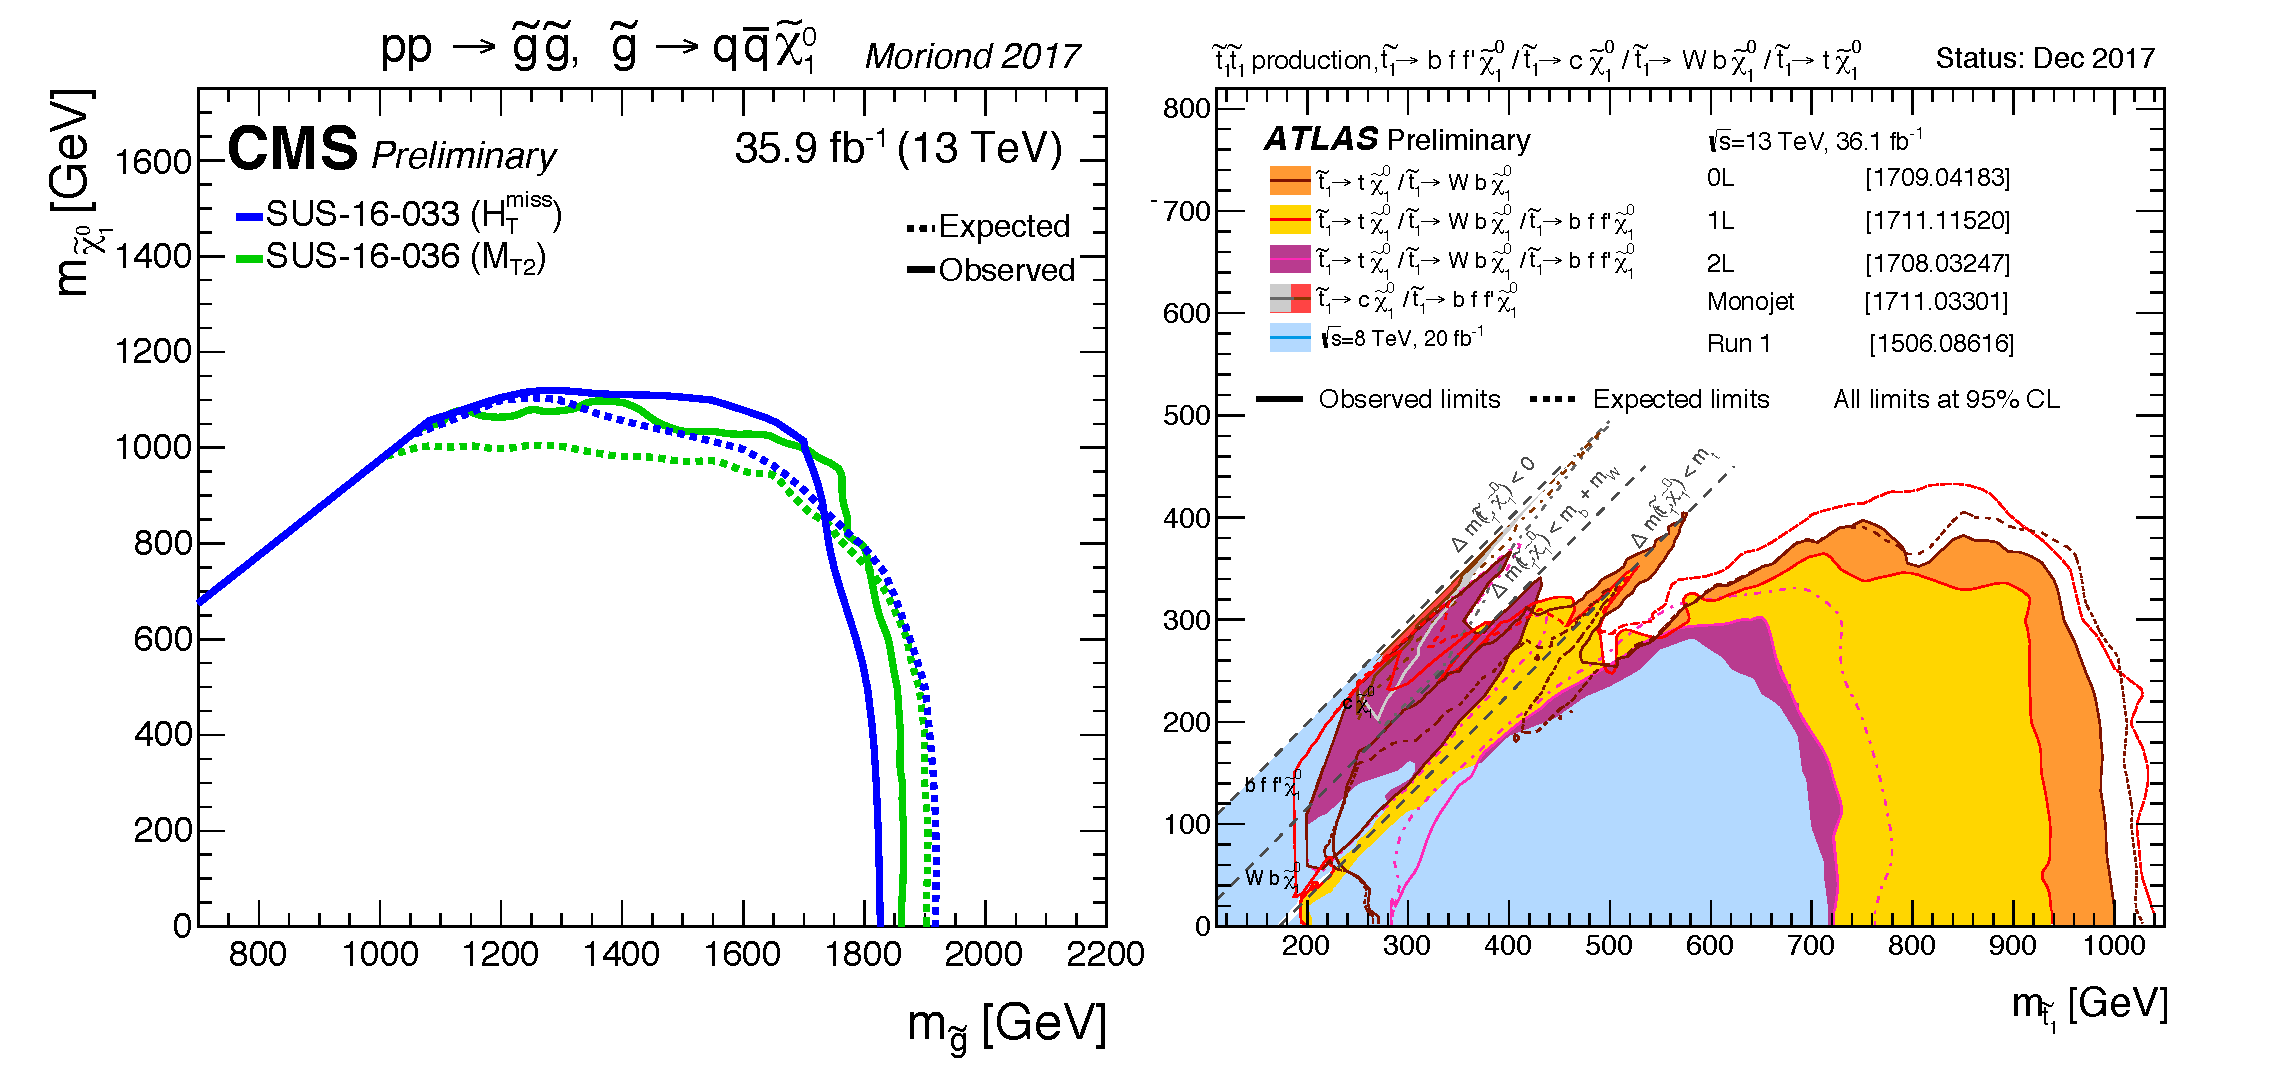
\includegraphics[width=\textwidth]{figures/SUSY_strong_ttbar.pdf}
%\caption{Mass reach of ATLAS and CMS searches for a selection of results targeting strongly produced SUSY particles, available as of December 2017. From~\cite{ATLASSUSYSummary,CMSSUSYSummary}.\label{fig:SUSYSummary_strong}}
%\end{figure}

No SUSY search so far has found evidence for new invisible particles, so limits can be set on the rates of SUSY processes. However, given the multitude of search channels and model points, it's difficult to make general statements about the current status, even for SUSY simplified models inspired by the MSSM. Perhaps the best one can say is that constraints from searches for strongly produced superpartners approach 2 TeV (see e.g.~\cite{Aaboud:2017bac,Sirunyan:2017yse}) for neutralino masses up to a TeV and, 
%https://twiki.cern.ch/twiki/pub/CMSPublic/PhysicsResultsSUS/T1tttt_limits_summary_cms_Moriond17.pdf
on the other hand, other processes are less constrained. For example, third-generation squarks, for which searches exploit final states with heavy flavor quarks, are generally only constrained to be at least several hundred GeV for neutralinos of similar masses, see e.g.~\cite{Sirunyan:2017wif,Aaboud:2016wna}.
% and Fig.~\ref{fig:SUSYSummary_strong}. 

%https://atlas.web.cern.ch/Atlas/GROUPS/PHYSICS/CombinedSummaryPlots/SUSY/ATLAS_SUSY_Stop_tLSP/ATLAS_SUSY_Stop_tLSP.png
%https://twiki.cern.ch/twiki/pub/CMSPublic/PhysicsResultsSUS/T2tt_limits_summary_cms_Moriond17.pdf

Direct production of weakly-coupled superpartners has a much smaller production rate, and hence the constraints on them are significantly weaker, as shown in Fig.~\ref{fig:SUSYSummary} (b). But, as shown in Figure~\ref{fig:SUSYSummary_strong}, there are numerous exceptions to these blanket statements, even before one remembers that the masses exclusions shown in the figure only apply to specific slices of a multi-dimensional model parameter space.

\begin{figure}[!htpb]
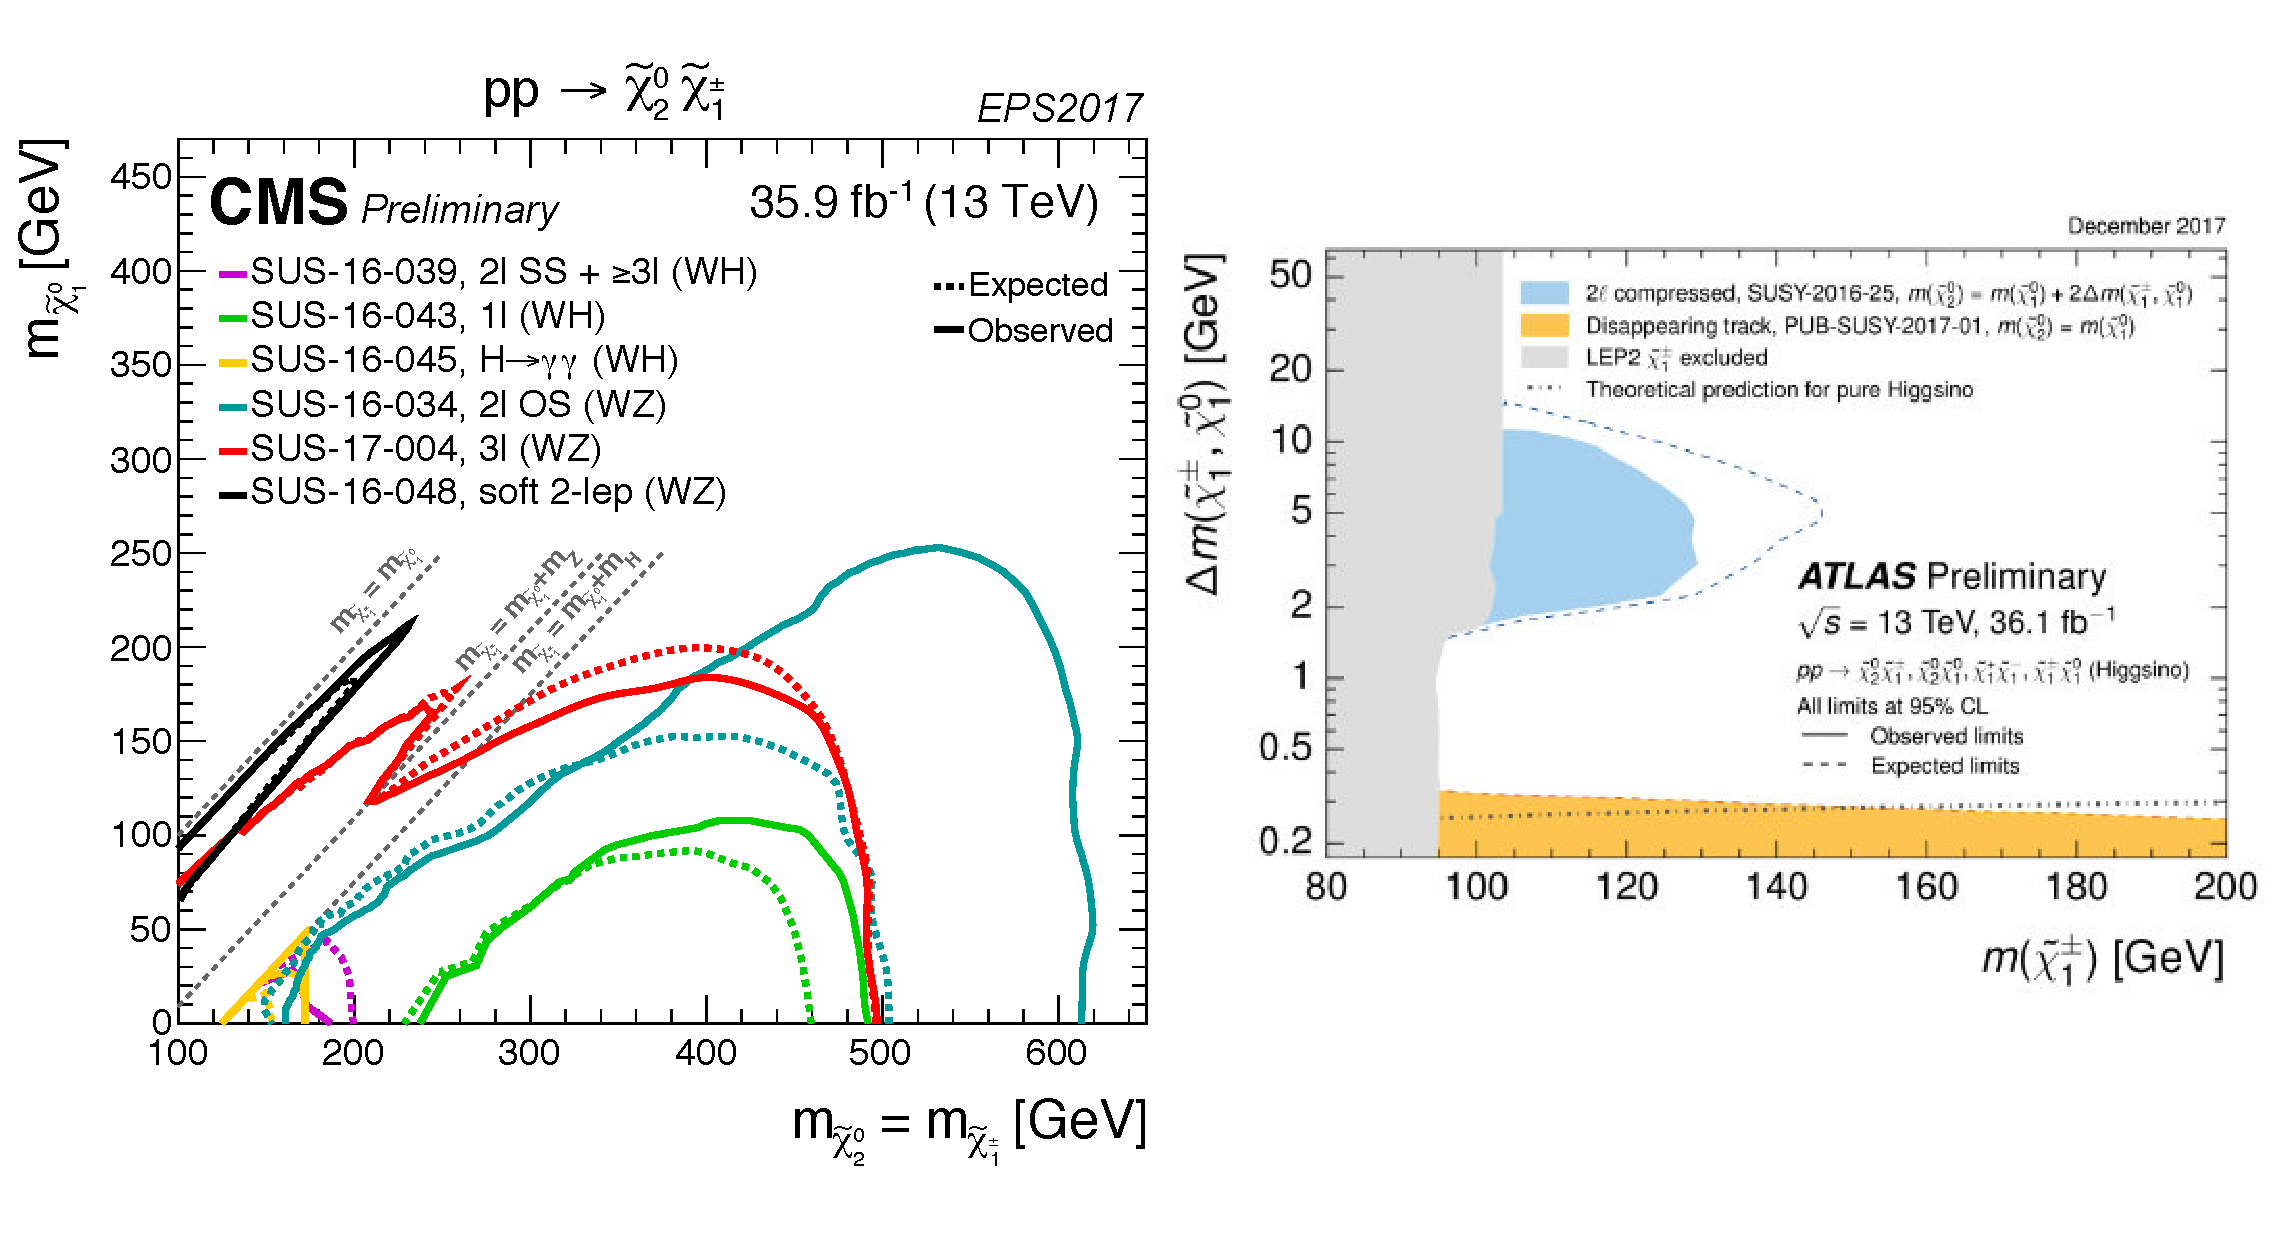
\includegraphics[width=\textwidth]{figures/SUSY_electroweak.pdf}
\caption{Mass reach of ATLAS and CMS searches for a selection of results targeting electroweak SUSY production, available as of December 2017. From~\cite{ATLASSUSYSummary,CMSSUSYSummary}.\label{fig:SUSYSummary_ew}}
\end{figure}

%https://atlas.web.cern.ch/Atlas/GROUPS/PHYSICS/CombinedSummaryPlots/SUSY/ATLAS_SUSY_EWSummary/ATLAS_SUSY_EWSummary.png

While, so far, the LHC searches have probed mainly strongly-produced SUSY channels, searches for rare processes are now entering their prime. With $36 \textrm{fb}^{-1}$ of data now collected, one can now begin to probe interesting parameter space for electroweakinos, by combining several channels as in~\cite{Sirunyan:2018ubx}. 
Searches for gauge boson superpartners (gauginos) have a reach of approximately 1 TeV if the superpartners of SM leptons are light and the search can benefit from a high leptonic branching ratio, while the constraint on the gaugino masses reduces to 600 GeV if their decays proceed through W and Z bosons. 
The larger luminosity also provides access to previously-inaccessible regions of parameter space for specific signatures, e.g. ``compressed'' regions where small superpartner mass differences lead to low \MET~\cite{Aaboud:2017leg}. 
Small mass differences can also suppress superpartner decays, resulting in long lifetimes that can then be exploited to study regions in which the mass splitting is as low as 0.2 GeV for Higgsino models~\cite{ATL-PHYS-PUB-2017-019}. 

%%SUSY scans

Targeting a specific signature, such as a cascade decay in a specific simplified SUSY model, drastically increases our ability to discover it. A narrower focus however trades generality for sensitivity, especially when interpreting results in terms of simplified models. 
%Designing and interpreting searches solely using simplified models may not capture the spectrum of possibilities
%given by full, theoretically well motivated models. 

Despite the diversity of possible SUSY signatures, a sufficiently specific SUSY model can provide a concrete framework on which to build an understanding of the combined effect of the many experimental constraints. Ref.\cite{Conley:2010du}, and continuing through LHC experiments ~\cite{Aad:2015baa, Khachatryan:2016nvf}, use the pMSSM to define a finite (though large) parameter space to probe. Though this approach does not provide rigid or exhaustive exploration of the possibilities, it can provide a coarse-grained map to identify under-examined signatures for future focus. Along with particle physics data, one may also add constraints identifying the LSP with astrophysical DM to further narrow this focus to particular regions compatible with a given cosmology, as in Ref.~\cite{Aaboud:2016wna} studying electroweakinos.
 %this is EW dark matter interpretations of ATLAS, maybe leave for comparisons section?

%Many tools (e.g. ) need to be combined to obtain these parameter scans. 
Collaborations such as GAMBIT~\cite{Athron:2017ard} and Mastercode~\cite{Bagnaschi:2017tru} have combined a variety of tools to aid building such maps. These codes encapsulate search results in statistical outputs which can be combined to construct global constraints for the invisible particle models of interest. 
An example are the likelihood functions for the viability of sets of parameters of a SUSY model given the available results from from both searches at colliders as well as Standard Model precision measurements and direct and indirect Dark Matter detection experiments.

\subsection{Searches in association with long-lived particles}
\label{sec:results_LLPSearches}

%unconventional reconstruction techniques
%- more eLLP phase space
%- disappearing tracks
%- compressed SUSY
%- dark boson models that are light because haven't seen heavy
%- detector signatures of dark bosons
%- dark photons
%- LHCb

%extreme range of experimental objects
So far, we've only discussed signatures of invisible particle production where the prompt decays produce visible recoil originating at the collision point. Long-lived intermediaries present different experimental challenges. 
For short lifetimes, the long-lived particles (LLP) will decay inside the tracking detectors, giving rise to displaced vertices. 
%need citation
Some SUSY decay chains (e.g. in split supersymmetry) can lead to disappearing tracks if visible particles decay into the LSP and soft particles~\cite{Aaboud:2017mpt}. 
%Another distinctive experimental signature of LLP is the "disappearing track", produced for example by SUSY models where a chargino
%with a short lifetime leaves a track in the inner detector which effectively disappears as it decays into a neutralino and a soft pion~\cite{Aaboud:2017mpt}. 
%disappearing track ATLAS
Longer-lived particles will decay in the calorimeters or in the muon spectrometers 
%need citation
or they may even exit the detector cavern completely before decaying. 
%need citation

These complications add yet another dimension of complexity to searches for these models, because even observing the events may require dedicated triggers, reconstruction algorithms, and even detectors\cite{Ball:2016zrp,Chou:2016lxi}. Nevertheless, these searches motivate specific, time-consuming detector and algorithms improvements, given that LHC searches didn't find any prompt new physics yet and given our ignorance of the dark sector and its interactions. 
%backgrounds generally small and instrumental (no SM), but difficult searches

After discussing supersymmetric models giving rise to long-lived particles in the previous section, we now focus on the results of a class of searches sensitive to very light dark vector and scalar bosons and their connection to the generic searches for prompt, high-mass vector and scalar mediators. 

%summary diagram in https://indico.cern.ch/event/656211/contributions/2673379/attachments/1498650/2333150/UW_dark_photons.pdf

% don't know where this goes
%The LHC searches mentioned in this chapter, with the exception of compressed SUSY scenarios, 
%so far target prompt production of WIMP invisible particles or associated mediator particles at colliders. 
%The absence of a signal constrains these traditional WIMP models to have small cross-sections and high mass scales. 
%This is one of the reasons why less-accessible dark boson and dark scalar models, including mediators with masses from the MeV to the tens
%of GeV and with a range of potential lifetimes, are a target that is gaining interest by LHC searches. A similar consideration
%applies for SUSY scenarios that are hard to detect. 
%These signatures are particularly challenging for ATLAS and CMS, given that many of these possibilities escape
%conventional detection.

Visible decays of light dark bosons have distinctive signatures, depending on their lifetime and couplings to the SM and dark sector. 

Oftentimes the dark boson is 

presence of the SM Higgs boson 

%vector, prompt (ATLAS Zd)
For visible decays of vector bosons
%vector non prompt (ATLAS prompt LJ)
%vector, prompt and non prompt (LHCb most stringent limits)

%scalar 
- does the dark boson decay into SM particles?
-- prompty
- does the dark boson decay invisibly?

%dark photon decaying in LJ
For example, the searches in~\cite{ATLAS:2016jza} look for \textit{lepton-jets}. These are collimated SM decay products of light,
long-lived boosted dark bosons that in turn are the exotic decay products of a SM Higgs connected to the dark sector. 

%H->dark bosons->LJ
This search constrains this kind of exotic Higgs decays to be below 10\% for a range of dark photon lifetimes. 

Other examples of searches for dark photons at general purpose experiments are through exotic decays of the Higgs boson~\cite{Aad:2015sva,CMS-PAS-HIG-16-035}, where dark bosons are pair-produced and each decay to muons. 

%visible decays of dark photon


%Prompt also exists, see Miriam's diagram
The BR of the SM Higgs boson is found to be below 10\% for a range of masses and lifetimes. 
This search benefits from tailored trigger and reconstruction algorithms for collimated muons. 

%The CMS mass range covered is 0.25-8.5 GeV, while the ATLAS range is 15 and 60 GeV
%Lepton-jets are also produced in SUSY cascade decays. 
%https://indico.cern.ch/event/492240/contributions/2302157/attachments/1367524/2072266/Leptonjets_HiggsCoupling_Nov2016_Safonov.pdf
%fun substructure for electron jets
%https://journals.aps.org/prd/abstract/10.1103/PhysRevD.95.055007
%If we want to mention sterile neutrinos (probably not), https://journals.aps.org/prd/abstract/10.1103/PhysRevD.91.093010
Drell-Yan dilepton production and electroweak precision observables are also sensitive to these models~\cite{Curtin:2014cca}, due to the mixing of the dark boson with the SM bosons. 
%Mention sensitivity? See Shelton's talk
The LHCb experiment can use precise tracking to search for visible decays of both prompt and long-lived dark vector bosons into muon pairs~\cite{Aaij:2017rft}, providing the most stringent constraints on dark bosons between 10 and 70 GeV. Dimuon pairs are also a decay signature for dark scalar particles with a long lifetime~\cite{Aaij:2016qsm}. %Results:
%Lifetimes of: 2�10?10 and 10?7
%masses of: No significant excess is observed in the accessible ranges of mass 250<m(?)<4700MeV/c2 and lifetime 0.1<?(?)<1000ps. 
LHCb is a non-hermetic forward experiment so it needs to rely on visible decays of the dark particles. 
Experiments at electron-positron colliders, such as the BaBar and Belle experiments, exploit the knowledge of the center-of-mass energy as a constraint to compensate their non-hermeticity, and set the most stringent collider limits on the kinetic coupling $\epsilon$ for this kind of models for dark boson masses between 0.5 and 10 GeV. 


%%%%%%%%
%ASSORTED JUNK
%%%%%%%%

%beginning with the searches that illustrate many of the experimental 
%
%
% and then signals of MET. 
%
% description has a historical and ordering
%We begin with introducing 
%
%start with introducing the searches, mostly  
%
% of invisible particles searches, we will turn to a [categorization] of the searches done so far. After a summary of searches for interactions through SM bosons, we turn to the experimental results 


%As described in the previous chapter, invisible particles itself is not visible at colliders and has
%to be observed indirectly in association with other visible particles. 
%
%Signals of invisible particles can come from MonoX and diX searches. 
%
%State of the art MC:
%
%Vector and scalar models are known at NLO~\cite{Neubert:2015fka,Haisch:2013ata}
%NLO corrections for vector and scalar models in monoZ and monojet
%
%t-channel
%
%From Millie's talk (see Reaction OmniOutliner):
%Since the invisible particles-mediator-quark vertices allow for simultaneous FS partons with different hard scale, particular prescription needs to be used for the generation of samples with different partons that splits samples in number of mediators. Interference between the diagrams is neglected following Papucci et al. 


\subsubsection{Consequences of neutral-mediated models: visible decays}
\label{sec:MediatorSearches}
\label{sub:twoBody}

%- coming from invisible particles: why would we do a search for visible particles and no invisible particles?
%- because colliders are probing the interactions with DM, not the DM
%-- to study the interaction, we don't need the DM to be produced
%-- e.g. it is possible to have very heavy DM and a much lighter mediator, in which case there would be no invisible particle signature at the collider, but we could still discover the mediator and study its properties.

%- as a specific example we take the s-channel model
%-- and the mediator has to decay into quarks and gluons and could decay in other visible particles as well
%-- because everyone loves resonances at hadron colliders, but high mass (give idea of how it's done)

%- results for low-mass
%-- problem: trigger thresholds
%-- solution: dijet+ISR (boosted/resolved) link to the previous ISR as object to tag events, TLA
%-- range of couplings constrained

%- complementarity between visible and invisible searches

So far, we have discussed searches for invisible particles as a tool to probe the interaction between the SM and the dark sector. 
However this interaction can be probed without actually producing the invisible particles. As an illustrative example for this section, if the mediator particle can be produced via interactions with quarks, it may also decay into quarks. 
In this case, searches sensitive to the visible signatures of (axial-)vector and axial vector models, namely dijet resonances (see e.g. ~\cite{Liew:2016oon,Fairbairn:2016iuf,Chala:2015ama}) [look for citations], can constrain the mediator.
%CD cite the following
%Coupling--mass mapping of di-jet peak searches, 10.1103/PhysRevD.88.035021 ok
%Searches for Dijet Resonances at Hadron Colliders, 10.1142/S0217751X11054905 in the experimental part, i would say
%Searching for Low Mass Dark Portal at the LHC, 10.1016/j.dark.2013.03.002 ok
%Constraining Dark Sectors with Monojets and Dijets, 10.1007/JHEP07(2015)089 ok
%Constraints on Z? models from LHC dijet searches and implications for invisible particles - https://arxiv.org/pdf/1605.07940.pdf -> ok

Dijet resonance searches have a long history at hadron colliders, where have been routinely used to probe the production of new particles at newly-reached collision energies~\cite{Harris:2011bh}. 
They exploit the absence of features in the falling QCD dijet invariant mass distribution to estimate its shape directly from a fit to those data, minimizing modelling and theory uncertainties. This permits the observation of low-rate localized excesses from resonant dijet production~\cite{Aaboud:2017yvp,CMS-PAS-EXO-16-056}. If the resonance is wider than 15\%, as in the case of 
vector and axial vector mediator models with couplings roughly above \gq$>$0.5~\footnote{This value
assumes that the new particle can decay only to quarks and invisible particles particles, with \gdm=1.0 and \mdm=1 GeV.}, the fitted background estimation may be biased by the presence of signal. Searches exploiting 
the scattering angle of dijet events are chosen to search for wider mediators decaying to dijets~\cite{CMS-PAS-EXO-16-046,Aaboud:2017yvp}. 

%Sidebar (50 words minimum, 200 words maximum) briefly discussing a fascinating adjacent topic; 
%insert below Literature Cited section, but indicate near which section in text the sidebar should be typeset
%Consider swapping with the ERC text below?
\begin{textbox}[!h]
\section{Selection of events at the detector level (trigger)}
%Trying to approximate 10 words per line
%Notes for improvement: 
%this is too long, needs sharpening. 
% the points i want to make are:
% higher thresholds are bad for mediator searches and also in general -> go TLA
% pileup increases MET thresholds -> get track info at the trigger level
%it needs a much clearer motivation: model X gives low mass. 
%probably that needs done in the text because space constraints, but then why using this box-thing (other than tidying things up)? 
The LHC collides protons every 25 $\mathrm{ns}$, producing 40 billion 
of events per second at nominal conditions. This amount of data cannot be 
recorded in its entirety, and not all events are interesting
for the experiments' physics programmes. %programmes or programs?
A trigger system is used to decide whether an event is selected for further analysis. 
Its first level is realized in hardware and only uses
partial detector information for fast decisions in a time of
the order of $\mathrm{\mu s}$, while its second level is software-based
and uses more refined algorithms and information to make a
decision in $\mathrm{ms}$. 

\textbf{Challenge: triggering on low-\pt objects}
Since the rates of SM physics processes decrease
with the transverse momentum of the objects involved, and processes
with a high momentum transfer have a higher chance of containing
interesting features or new particles, the trigger system records
events above a certain threshold e.g. in leading jet \pt or in event \MET. 
Only a fraction of events that do not satisfy these thresholds is recorded. 
Searches for signals with high-rate backgrounds and 
MET or jet \pt below these thresholds are 
therefore penalized unless novel
%not novel anymore?
data recording techniques, such as only recording partial event information 
needed for the search, are employed.

\textbf{Challenge: \textit{pile-up} in trigger} Simultaneous proton-proton interactions occurring within the detector
readout time cannot be completely disentangled from the hard process
of interest, especially if reconstructing the collision vertex
is not possible at the trigger level due to CPU constraints. 
This \textit{pile-up} increases the likelihood of passing 
the minimum threshold to record events, especially in the \MET triggers.
For this reason, the increase in the LHC instantaneous luminosity by virtue
of increasing the number of simultaneous
collisions leads to increases in the trigger thresholds to
keep manageable event recording rates. Reconstruction algorithms that suppress
the effects of pile-up can be employed by ATLAS and CMS directly at the trigger level,
using information on the objects and energy density within the event~\cite{CMS:2014ata,ATLAS-CONF-2014-019}. 
In future LHC runs, track information to disentangle the provenance of the 
energy deposits from the collision vertex will be available for
ATLAS and CMS from dedicated hardware systems (see e.g. Refs.~\cite{Shochet:2013gaw,1748-0221-6-12-C12065}). 
\end{textbox}


%Where dijets lose sensitivity: low-mass 
Standard LHC dijet searches lose sensitivity at masses below the TeV~\cite{An:2012ue,Dobrescu:2013coa}, where the high QCD rates force the experiments to randomly discard a large fraction of background and signal events alike. 
Recording only final state objects reconstructed within the trigger system~\cite{Aaij:2016rxn,CMS-PAS-EXO-16-056,Aaboud:2016leb} is a way to overcome the limitation due to the limited storage for QCD-like events at low invariant masses and be sensitive to mediators with masses
above 400 GeV~\cite{CMS-PAS-EXO-16-056,ATLAS:2016xiv}. 
An alternative data-taking strategy is to require a high-\pt{} ISR object recoiling against the dijet pair to reduce the QCD background, in the same spirit as for the jet and photon+\MET searches above~\cite{ATLAS:2016bvn,Sirunyan:2017nvi}. The lowest mediator masses are reached by searches exploiting substructure techniques when the mediator is boosted and its decay products are collimated~\cite{Sirunyan:2017nvi}.
[add ATLAS boosted]
Searches for \textbf{$b\bar{b}$ or $t\bar{t}$ resonances}~\cite{lowMassDiB,CMS-PAS-HIG-16-025,Aaboud:2017hnm} are sensitive to
mediator particles decaying democratically to different quark flavours or preferentially into heavy flavour quarks (as in the case for a scalar mediator).

If the interaction between SM and dark sector includes leptons, LHC dilepton search are sensitive to even lighter mediators~\cite{Aaboud:2017buh,Khachatryan:2016zqb}. 
The main backgrounds for the dilepton searches in electron and muon final states arise from Drell-Yan processes, and are estimated using simulation corrected for NNLO effects and normalized to the Z boson peak event yield in data. For this reason, the dominant uncertainties on the background estimation are of theoretical nature. 
%ATLAS. too much detail
%The background prediction is smoothed using functional fits where the number of simulated events is not representative of the data statistics. 
%Reducible backgrounds where other objects are mismeasured as leptons are estimated using data. The main uncertainties on the background estimation are of theoretical nature, for the entire invariant mass range. 

%Even though lepton couplings are not mandated by the quark-antiquark production at hadron colliders as dijet couplings are, 
%lepton couplings feature in a variety of models that can embed the simplified models of invisible particles used as benchmark for LHC searches. %this sentence repeats the one in Sec.2. 

%results

[add coupling-mass summary plot?]

Having observed no excess, the constraints on the interaction rates for (axial-)vector models can be translated into limits on the couplings of the mediator with SM particles at given mediator and invisible particle masses. 
%List constraints from both searches with two coupling options
%The CMS analysis also scans the coupling-mass plane by fixing the ratio between \minvisible particles and \mmed to ensure perturbativity 
%CMS sentence: Quark couplings down to 0.05 for mediator masses at 50 GeV are excluded for the spin- 1 simplified models as shown in Fig. 12. 
The same constraints from dijet and dilepton searches apply to both vector and axial vector mediators: the LHC phenomenology (rates and kinematics) is the same for both. 
Searches for visible mediator decays are sensitive to masses as low as 50 GeV (boosted dijet+ISR) and constrain SM-invisible particles couplings \gq as low as 0.06 at 60 GeV. Jets from the mediator decay start being spatially separated above mediator masses of 250-300 GeV, where the $\gamma$ and gluon ISR + dijet channel constrain \gq$>$0.15-0.2. Searches with jets at the trigger level are the most sensitive to low-mass mediators where results are available, excluding simplified models with \gq as low as 0.05 starting from 400 GeV. Above the TeV, standard dijet resonance and angular searches constrain quark couplings from 0.1 to unity, up to 5 TeV. 
%but lose sensitivity to lower couplings where they start to be statistically limited. 
Dilepton searches are more sensitive than dijet searches in case of equal couplings of the mediator to leptons and jets, due to the much reduced backgrounds. ATLAS and CMS searches with the 2015+2016 dataset probe signal masses starting from 150 and 400 GeV respectively. 
%what is the minimum coupling by dilepton searches? not sure this is easy to do without reinterpretation

%Mention LianTao's paper where baryonic / 2Hinvisible particles monoHiggs is also constrained. 
%Mention results of other searches: ttbar resonances for pseudoscalar with interference, Higgs-like scalars (CMS boosted) 


\subsubsection{Comparison of sensitivity of visible and invisible LHC searches}
\label{sub:comparisonVisibleInvisible}

%- General thing
When searches can directly target specific, fully-visible signatures of a particular dark interaction, they can be powerful probes of that interaction, and in some cases (e.g., when the invisible particles are too heavy to be directly produced) are the only way to observe dark interactions at a collider. On the other hand, only \MET searches can observe the invisible particle production directly. Each type of search complements the others; nevertheless, piecing together searches in different channels requires a model---a model which may have many degrees of freedom---and so understanding precisely how these searches fit together can be challenging when little is known about dark interactions.

%- as an example for comparison of visible and invisible searches only covering a specific model, behold the summary plots
%- showing the relative power of these searches
%- mention DMWG (sidebox?) so the reader can get involved or have questions
To understand how this could work in practice, we again consider the case of (axial-)vector mediators, to which both jet+\MET and two-body resonance searches are sensitive. Even though the model is simple, its parameter space is four-dimensional (couplings, invisible particle mass, mediator mass), and different projections can be used to display results. The two-dimensional plane chosen to present results of visible and invisible particle searches, after discussion of the experimental and theory community interested in DM searches (called Dark Matter Working Group) is that of mediator mass and DM mass~\footnote{This is following the SUSY convention of presenting search results in the plane of neutralino mass against superpartner particle mass}, with fixed coupling values. The constraints from the different searches are displayed as excluded points in this plane, and the models parameters are clearly specified on the plots themselves.  

The coupling parameter values used as benchmarks have been selected considering the sensitivity of early Run-2 searches, precision constraints and general simplicity arguments, as well as the desire to showcase the complementarity of different LHC searches. The basic scenario for vector and axial vector searches is that of a mediator that only couples to quarks, with \gq=0.25, \gl=0. and \gdm=1. This is complemented by a scenario where couplings to quarks are reduced to 0.1, decreasing both production and visible decay, and scenarios where lepton couplings are present. Figure~\label{fig:sensitivityComparison} shows the results of LHC searches corresponding to two of these scenarios. The left-hand plot shows a leptophobic vector mediator with \gl=0, \gdm=1.0 and \gq=0.25, where dijet searches for visible decays of the mediator constrain both on-shell and off-shell region but are limited by data-taking constraints at masses above roughly 50 GeV, where \MET+X searches take over in the on-shell region. 
%An equivalent picture is drawn for the vector mediator, in the top right plot. The bottom right plot shows the case of an axial vector mediator with reduced quark couplings and equal lepton couplings (\gq=\gl=0.1 and \gdm=1.0), where 
The right plot shows the scenario of a vector mediator where both lepton and quark couplings are reduced with respect to the previous scenario, and lepton couplings are smaller than quark couplings (\gq=0.1, \gl=0.01, \gdm=1.0). 
The range of all regions constrained by dijet decays of the mediator is considerably reduced with respect to the scenarios with larger couplings. Searches for dilepton resonances cover a larger range of parameter space with respect to dijet resonances but are still limited at mediator masses below 100 GeV, where \MET+jet searches are still sensitive. 

%; the region constrained by from \MET+jet searches extends to lower invisible particles and mediator masses with respect to the case of the model with \gq=0.25 due to the reduced production rate. 

%TODO: make more visible, limit to 2 plots only top left and bottom right
\begin{figure}[!htpb]
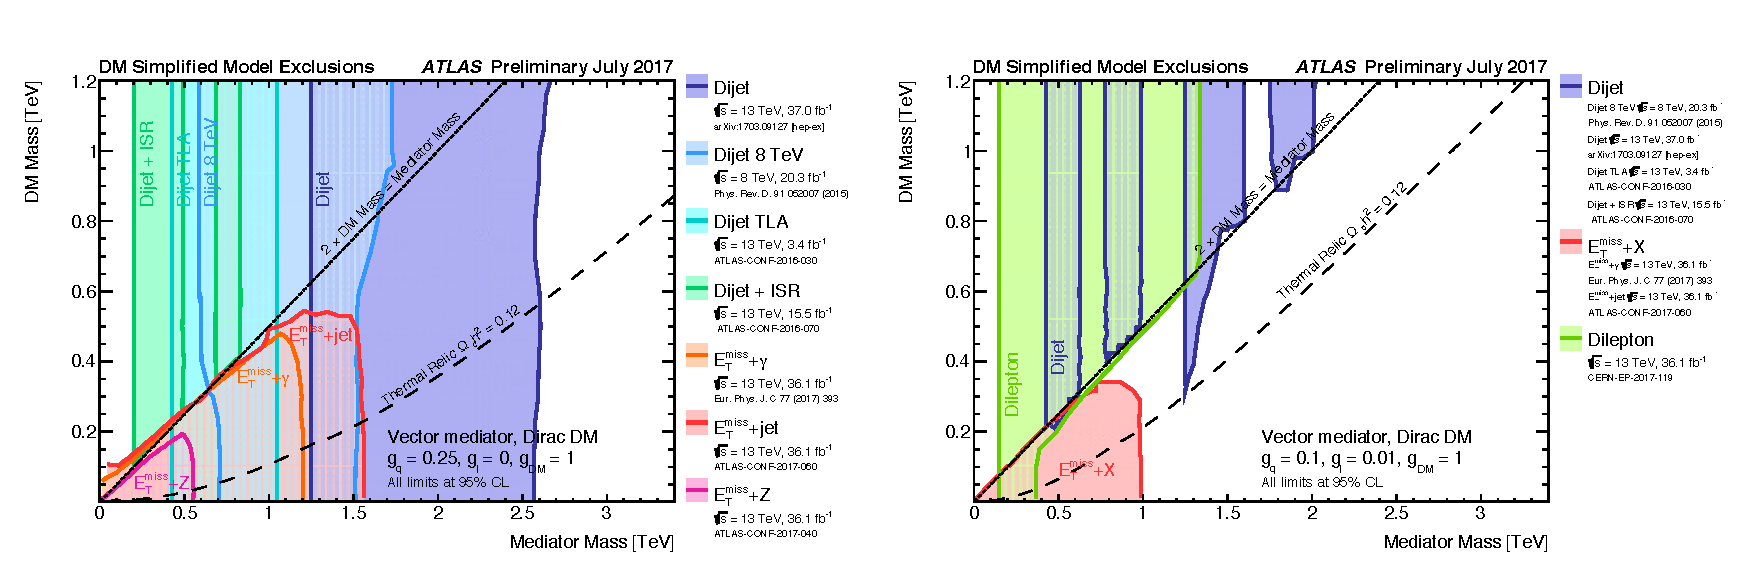
\includegraphics[width=\textwidth]{figures/SummaryPlotsMassMass.pdf}\caption{
Regions in a dark matter mass-mediator mass plane excluded at 95\% CL by a selection of ATLAS dark matter searches, for a vector mediator benchmark model with varying coupling scenarios. Top plots: \gq=0.25, \gl=0.0, \gdm=1.0, axial vector (left, separate search constraints) and vector mediator (right, combined search constraints), highlighting the sensitivity of visible searches in this scenario and the near-equivalence of the vector and axial vector as benchmark models for LHC searches. Bottom plots: \gq=0.1, \gl=0.1, \gdm=1.0 for an axial vector mediator (left) and \gq=0.1, \gl=0.01, \gdm=1.0 for a vector mediator (right), highlighting the sensitivity of the lepton searches and its dependence on the chosen coupling value. Dashed curves labeled "thermal relic" indicate combinations of dark matter and mediator mass that are consistent with a dark matter density of $\omega_c = 0.12 h^2$ and a standard thermal history, as computed in MadDM particles~\cite{Backovic:2015cra}. The dotted curve indicates the kinematic threshold where the mediator can decay on-shell into dark matter. }
%\gdm=1.0  \gq=0.25universal to all flavors, and a lepton coupling gl set to zero. This choice of couplings corresponds to the "V1" scenario in arXiv:1703.05703. Leptonic decays are absent at tree level. The results use 13 TeV data except for Phys. Rev. D91 052007 (2015). The exclusions from the ATLAS dijet searches are derived from the limits provided on Gaussian-shaped resonances following the procedure recommended by ATLAS in Appendix A of Phys. Rev. D91 052007 (2015) and in arXiv:1703.09127. Small fluctuations in the contour are a product of the dijet reinterpretation scheme. 
%To the left of the curve, annihilation processes described by the simplified model deplete ?c below 0.12 h2. A dotted curve indicates the kinematic threshold where the mediator can decay on-shell into dark matter. The exclusion regions, relic density contours, and unitarity curve are not applicable to other choices of coupling values or model.
\label{fig:sensitivityComparison}
\end{figure}


%It is important to note that generic searches for new two-body resonances are by design sensitive to a broad range of theoretical benchmarks, 
%and as such they alone can offer little information on whether a discovery would imply in terms of invisible particles mediators.

%- narrate coupling dependence
%- point out that when visible searches more specifically target the mediator, and when the invisible particle cannot be produced because too heavy, they are more powerful than generic searches
%- pitfalls: they can't go as low in mMed or m invisible as invisible searches (that only uses more boosted MET)
%-- one cannot generalize about DM from a single simplified model, different production mechanism
%-- the interaction is ruled out for a particular DM mass

These plots show that the relative sensitivity of visible and invisible searches is a model- and parameter-dependent statement. For $s-$channel simplified models where the couplings to SM are not negligible compared to the dark sector coupling, visible searches that more specifically target the mediator are more constraining than their invisible counterparts, in particular if the invisible particle is heavy and cannot be produced at the collider. 
%Invisible particle searches however would dominate whenever the 
%for invisible particles only dominate if the coupling to invisible particles is much larger than the coupling to quarks, and even then reducing \gq reduces the LHC production cross-section and therefore the overall sensitivity of \MET+X searches. When visible searches 
One advantage of searches for invisible particles is their sensitivity to models with very light mediators ($<$50 GeV) and light \mdm, since the reach of dijet and dilepton searches to low-mass resonances is still ultimately limited by data taking constraints. 
%In absence of a signal and within a specific model scenario, searches for mediator particle with visible decays provide constraints that are complementary to those of searches for invisible particles, in particular in the off-shell region 2\mdm $>$ \mmed where the mediator cannot decay to invisible particles directly but can still decay into much lighter SM particles such as leptons and quarks. 

[redundancy check?]
We finally remark again that none of these results rule out invisible particles with a given mass; they rule out {\it interactions} with invisible particles of that mass.

%- pitfalls: they can't go as low in mMed or m invisible as invisible searches (that only uses more boosted MET)
%-- one cannot generalize about DM from a single simplified model, different production mechanism
%-- the interaction is ruled out for a particular DM mass

%Mention why we plot things in the mass-mass plane. 
%A sketch of the comparison of the sensitivity of searches for visible decays of vector and axial vector mediator models, and invisible particles 
%in the \minvisible particles vs \mmed plane is shown in Fig.~\ref{fig:sensitivityComparison}, fixing the couplings. The choice of plane and the scenarios chosen follow the choices of the Dark Matter Working Group~\cite{Albert:2017onk}, to illustrate the complementarity of different LHC searches for $s-$channel-mediated model of invisible particles and to convey the message that the sensitivity of LHC searches to simplified models of invisible particles depends both on model choice and parameter choice. 
%Mention why mass-mass? Because on-shell/off-shell regions clearly spelled out

%Couplings for vector and axial-vector mediated models 

%results are given in the \mdm particles, \mmed  plane fixing the couplings to \gq=0.25 and \gdm particles=1.0 for vector and axial vector mediated models, \gq=\gdm particles=1.0 for scalar and pseudoscalar models and \gdm particlesq=1.0 for colored scalar models. The simplified models employed by the experimental collaborations are known at NLO~\cite{Neubert:2015fka,Haisch:2013ata,Backovic:2015soa}. 

%- putting things together in a global picture is hard, lots of parameters and so forth
%-- there's a 4D param space even in the simplest models

%CD: if we want coupling-mass, we could show the plots in the figs dir: SummaryPlotsCouplingMass.pdf

%In case sample figure with different scenarios as an example
%\begin{figure}[!htpb]
%\includegraphics[width=\textwidth]{figures/invisible particlesSummary.png}
%\caption{Illustrative examples of the comparison of the sensitivity of searches for visible and invisible mediators in the \minvisible particles-\mmed plane, for different coupling scenarios. No actual data has been used, but experimental observations have been used as inspiration for the figure. From~\cite{AnotherWikipedia}.}
%\label{fig:sensitivityComparison}
%\end{figure}

%It would be nice to make tables of lowest mediator/invisible particles searches+refs for 100 GeV invisible particles mass,
%as a poor-person approximation of a summary plot we can't make because ATLAS data not public. 

%%%SUMMARY TABLE FOR MONOX SEARCHES: descoped, unless we just want a list of references of all the searches which may be useful but obsoletes early
%\begin{table}[h]
\tabcolsep7.5pt
\caption{Summary of searches for BSM mediators at the LHC}
\label{tab:BSMSearchesSummary}
\begin{center}
\begin{tabular}{@{}l|c|c|c|c@{}}
\hline
Signature & Model& \mmed limit & \mdm limit  & Cit.\\
 &  & (\mdm=100 GeV) & (\mmed=100 GeV)  &  \\
%{(}units)$^{\rm a}$ &Head 2 &Head 3 &Head 4 &{(}units)\\
\hline
Jets+\MET & $s-$channel, AV$^{\rm a}$ & Column3 & Column4 & \cite{Sirunyan:2017jix,Aaboud:2017phn} \\
Jets+\MET & $s-$channel, V$^{\rm a}$ & Column3 & Column4 & \cite{Sirunyan:2017jix,Aaboud:2017phn} \\
Jets+\MET & colored scalar & Column3 & Column4 & \cite{Sirunyan:2017jix,Aaboud:2017phn} \\
Photon+\MET & Column 2 & Column3 & Column4 & Column\\
W,Z (had)+\MET 1 & Column 2 & Column3 & Column4 &Column\\
W,Z (lep)+\MET 1 & Column 2 & Column3 & Column4 &Column\\
Higgs+\MET &Column 2 & Column3 & Column4 &Column\\
\hline
\end{tabular}
\end{center}
%\begin{tabnote}
$^{\rm a}$ Coupling values: \gq=0.25, \gdm=1.0; $^{\rm b}$second table footnote.
%\end{tabnote}
\end{table}



